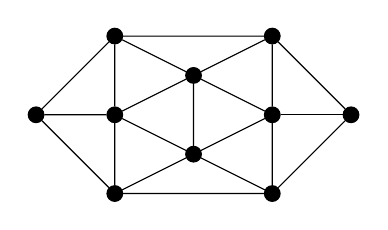
\begin{tikzpicture}[every node/.style={draw,inner sep=2pt,fill=black}]
      \path[shape=circle]
	(0,1) node(a1){} 
	(1,0) node(b1){} (1,1) node(b2){} (1,2) node(b3){}
	(2,0.5) node(c1){} (2,1.5) node(c2){}
	(3,0) node(d1){} (3,1) node(d2){} (3,2) node(d3){}
	(4,1) node(e1){};
	\filldraw (a1) -- (b1) -- (d1) -- (e1) -- (d3) -- (b3) -- (a1) -- (b2);
	\filldraw (b1) -- (b2) -- (b3) -- (c2) -- (d3) -- (d2) -- (d1) -- (c1) -- (b1);
	\filldraw (c1) -- (b2) -- (c2) -- (c1);
	\filldraw (c1) -- (d2) -- (c2);
	\filldraw (d2) -- (e1);
    \end{tikzpicture}